\documentclass[14pt]{extbook}
\usepackage{multicol, enumerate, enumitem, hyperref, color, soul, setspace, parskip, fancyhdr} %General Packages
\usepackage{amssymb, amsthm, amsmath, latexsym, units, mathtools} %Math Packages
\everymath{\displaystyle} %All math in Display Style
% Packages with additional options
\usepackage[headsep=0.5cm,headheight=12pt, left=1 in,right= 1 in,top= 1 in,bottom= 1 in]{geometry}
\usepackage[usenames,dvipsnames]{xcolor}
\usepackage{dashrule}  % Package to use the command below to create lines between items
\newcommand{\litem}[1]{\item#1\hspace*{-1cm}\rule{\textwidth}{0.4pt}}
\pagestyle{fancy}
\lhead{Progress Quiz 8}
\chead{}
\rhead{Version ALL}
\lfoot{5493-4176}
\cfoot{}
\rfoot{Summer C 2021}
\begin{document}

\begin{enumerate}
\litem{
To estimate the one-sided limit of the function below as $x$ approaches 2 from the left, which of the following sets of numbers should you use?\[ \frac{\frac{2}{x} - 1}{x - 2} \]\begin{enumerate}[label=\Alph*.]
\item \( \{ 2.0000, 2.1000, 2.0100, 2.0010 \} \)
\item \( \{ 2.0000, 1.9000, 1.9900, 1.9990 \} \)
\item \( \{ 1.9000, 1.9900, 2.0100, 2.1000 \} \)
\item \( \{ 2.1000, 2.0100, 2.0010, 2.0001 \} \)
\item \( \{ 1.9000, 1.9900, 1.9990, 1.9999 \} \)

\end{enumerate} }
\litem{
Based on the information below, which of the following statements is always true?
\begin{center}
    \textit{ $f(x)$ approaches $\infty$ as $x$ approaches $3$. }
\end{center}
\begin{enumerate}[label=\Alph*.]
\item \( f(x) \text{ is close to or exactly } \infty \text{ when } x \text{ is large enough}. \)
\item \( f(x) \text{ is close to or exactly } 3 \text{ when } x \text{ is large enough}. \)
\item \( f(x) \text{ is undefined when } x \text{ is close to or exactly } 3. \)
\item \( x \text{ is undefined when } f(x) \text{ is close to or exactly } \infty. \)
\item \( \text{None of the above are always true.} \)

\end{enumerate} }
\litem{
To estimate the one-sided limit of the function below as $x$ approaches 4 from the left, which of the following sets of numbers should you use?\[ \frac{\frac{4}{x} - 1}{x - 4} \]\begin{enumerate}[label=\Alph*.]
\item \( \{ 3.9000, 3.9900, 3.9990, 3.9999 \} \)
\item \( \{ 3.9000, 3.9900, 4.0100, 4.1000 \} \)
\item \( \{ 4.0000, 3.9000, 3.9900, 3.9990 \} \)
\item \( \{ 4.1000, 4.0100, 4.0010, 4.0001 \} \)
\item \( \{ 4.0000, 4.1000, 4.0100, 4.0010 \} \)

\end{enumerate} }
\litem{
Evaluate the one-sided limit of the function $f(x)$ below, if possible.\[ \lim_{x \rightarrow 7^+} \frac{-9}{(x+7)^3}+4 \]\begin{enumerate}[label=\Alph*.]
\item \( f(7) \)
\item \( -\infty \)
\item \( \infty \)
\item \( \text{The limit does not exist} \)
\item \( \text{None of the above} \)

\end{enumerate} }
\litem{
For the graph below, find the value(s) $a$ that makes the statement true: $ \displaystyle \lim_{x \rightarrow a} f(x)$ does not exist.
\begin{center}
    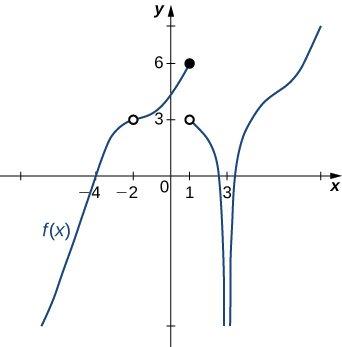
\includegraphics[width=0.5\textwidth]{../Figures/evaluateLimitGraphicallyCopyA.png}
\end{center}
\begin{enumerate}[label=\Alph*.]
\item \( 3 \)
\item \( 1 \)
\item \( -2 \)
\item \( \text{Multiple } a \text{ make the statement true}. \)
\item \( \text{No } a \text{ make the statement true}. \)

\end{enumerate} }
\litem{
Based on the information below, which of the following statements is always true?
\begin{center}
    \textit{ $f(x)$ approaches $13.648$ as $x$ approaches $1$. }
\end{center}
\begin{enumerate}[label=\Alph*.]
\item \( f(13) = 1 \)
\item \( f(13) \text{ is close to or exactly } 1 \)
\item \( f(1) = 13 \)
\item \( f(1) \text{ is close to or exactly } 13 \)
\item \( \text{None of the above are always true.} \)

\end{enumerate} }
\litem{
Evaluate the one-sided limit of the function $f(x)$ below, if possible.\[ \lim_{x \rightarrow 7^+} \frac{-1}{(x+7)^3}+7 \]\begin{enumerate}[label=\Alph*.]
\item \( -\infty \)
\item \( \infty \)
\item \( f(7) \)
\item \( \text{The limit does not exist} \)
\item \( \text{None of the above} \)

\end{enumerate} }
\litem{
Evaluate the limit below, if possible.\[ \lim_{x \rightarrow 7} \frac{\sqrt{7x - 24} - 5}{6x - 42} \]\begin{enumerate}[label=\Alph*.]
\item \( 0.100 \)
\item \( 0.017 \)
\item \( \infty \)
\item \( 0.117 \)
\item \( \text{None of the above} \)

\end{enumerate} }
\litem{
Evaluate the limit below, if possible.\[ \lim_{x \rightarrow 9} \frac{\sqrt{9x - 65} - 4}{3x - 27} \]\begin{enumerate}[label=\Alph*.]
\item \( 1.000 \)
\item \( 0.125 \)
\item \( 0.042 \)
\item \( \infty \)
\item \( \text{None of the above} \)

\end{enumerate} }
\litem{
For the graph below, find the value(s) $a$ that makes the statement true: $ \displaystyle \lim_{x \rightarrow a} f(x)$ does not exist.
\begin{center}
    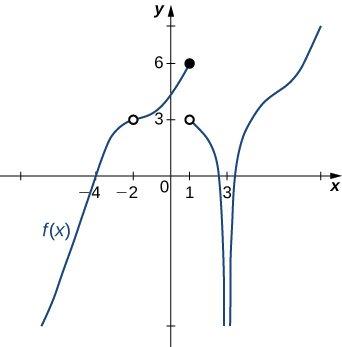
\includegraphics[width=0.5\textwidth]{../Figures/evaluateLimitGraphicallyA.png}
\end{center}
\begin{enumerate}[label=\Alph*.]
\item \( -2 \)
\item \( 1 \)
\item \( 3 \)
\item \( \text{Multiple } a \text{ make the statement true}. \)
\item \( \text{No } a \text{ make the statement true}. \)

\end{enumerate} }
\litem{
To estimate the one-sided limit of the function below as $x$ approaches 6 from the right, which of the following sets of numbers should you use?\[ \frac{\frac{6}{x} - 1}{x - 6} \]\begin{enumerate}[label=\Alph*.]
\item \( \{ 5.9000, 5.9900, 5.9990, 5.9999 \} \)
\item \( \{ 6.0000, 6.1000, 6.0100, 6.0010 \} \)
\item \( \{ 5.9000, 5.9900, 6.0100, 6.1000 \} \)
\item \( \{ 6.1000, 6.0100, 6.0010, 6.0001 \} \)
\item \( \{ 6.0000, 5.9000, 5.9900, 5.9990 \} \)

\end{enumerate} }
\litem{
Based on the information below, which of the following statements is always true?
\begin{center}
    \textit{ $f(x)$ approaches $\infty$ as $x$ approaches $4$. }
\end{center}
\begin{enumerate}[label=\Alph*.]
\item \( f(x) \text{ is close to or exactly } \infty \text{ when } x \text{ is large enough}. \)
\item \( f(x) \text{ is close to or exactly } 4 \text{ when } x \text{ is large enough}. \)
\item \( f(x) \text{ is undefined when } x \text{ is close to or exactly } 4. \)
\item \( x \text{ is undefined when } f(x) \text{ is close to or exactly } \infty. \)
\item \( \text{None of the above are always true.} \)

\end{enumerate} }
\litem{
To estimate the one-sided limit of the function below as $x$ approaches 1 from the left, which of the following sets of numbers should you use?\[ \frac{\frac{1}{x} - 1}{x - 1} \]\begin{enumerate}[label=\Alph*.]
\item \( \{ 0.9000, 0.9900, 1.0100, 1.1000 \} \)
\item \( \{ 0.9000, 0.9900, 0.9990, 0.9999 \} \)
\item \( \{ 1.0000, 1.1000, 1.0100, 1.0010 \} \)
\item \( \{ 1.0000, 0.9000, 0.9900, 0.9990 \} \)
\item \( \{ 1.1000, 1.0100, 1.0010, 1.0001 \} \)

\end{enumerate} }
\litem{
Evaluate the one-sided limit of the function $f(x)$ below, if possible.\[ \lim_{x \rightarrow 7^+} \frac{5}{(x+7)^4}+9 \]\begin{enumerate}[label=\Alph*.]
\item \( f(7) \)
\item \( \infty \)
\item \( -\infty \)
\item \( \text{The limit does not exist} \)
\item \( \text{None of the above} \)

\end{enumerate} }
\litem{
For the graph below, find the value(s) $a$ that makes the statement true: $ \displaystyle \lim_{x \rightarrow a} f(x) = 0$.
\begin{center}
    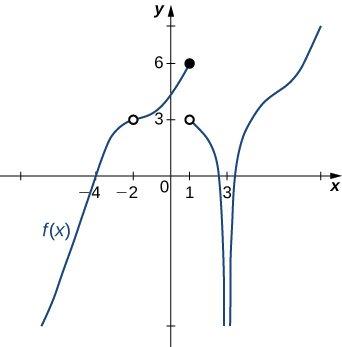
\includegraphics[width=0.5\textwidth]{../Figures/evaluateLimitGraphicallyCopyB.png}
\end{center}
\begin{enumerate}[label=\Alph*.]
\item \( 0 \)
\item \( 3 \)
\item \( -4 \)
\item \( \text{Multiple } a \text{ make the statement true}. \)
\item \( \text{No } a \text{ make the statement true}. \)

\end{enumerate} }
\litem{
Based on the information below, which of the following statements is always true?
\begin{center}
    \textit{ $f(x)$ approaches $19.045$ as $x$ approaches $8$. }
\end{center}
\begin{enumerate}[label=\Alph*.]
\item \( f(19) \text{ is close to or exactly } 8 \)
\item \( f(19) = 8 \)
\item \( f(8) = 19 \)
\item \( f(8) \text{ is close to or exactly } 19 \)
\item \( \text{None of the above are always true.} \)

\end{enumerate} }
\litem{
Evaluate the one-sided limit of the function $f(x)$ below, if possible.\[ \lim_{x \rightarrow 6^-} \frac{-8}{(x-6)^3}+2 \]\begin{enumerate}[label=\Alph*.]
\item \( -\infty \)
\item \( f(6) \)
\item \( \infty \)
\item \( \text{The limit does not exist} \)
\item \( \text{None of the above} \)

\end{enumerate} }
\litem{
Evaluate the limit below, if possible.\[ \lim_{x \rightarrow 4} \frac{\sqrt{7x - 3} - 5}{2x - 8} \]\begin{enumerate}[label=\Alph*.]
\item \( \infty \)
\item \( 1.323 \)
\item \( 0.050 \)
\item \( 0.100 \)
\item \( \text{None of the above} \)

\end{enumerate} }
\litem{
Evaluate the limit below, if possible.\[ \lim_{x \rightarrow 7} \frac{\sqrt{5x - 10} - 5}{3x - 21} \]\begin{enumerate}[label=\Alph*.]
\item \( 0.100 \)
\item \( 0.745 \)
\item \( \infty \)
\item \( 0.033 \)
\item \( \text{None of the above} \)

\end{enumerate} }
\litem{
For the graph below, find the value(s) $a$ that makes the statement true: $ \displaystyle \lim_{x \rightarrow a} f(x)$ does not exist.
\begin{center}
    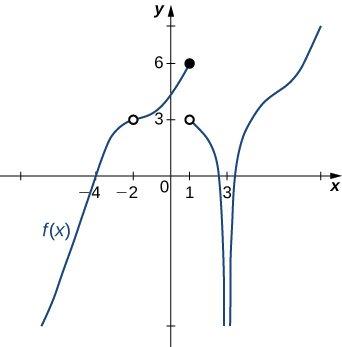
\includegraphics[width=0.5\textwidth]{../Figures/evaluateLimitGraphicallyB.png}
\end{center}
\begin{enumerate}[label=\Alph*.]
\item \( 1 \)
\item \( 3 \)
\item \( -2 \)
\item \( \text{Multiple } a \text{ make the statement true}. \)
\item \( \text{No } a \text{ make the statement true}. \)

\end{enumerate} }
\litem{
To estimate the one-sided limit of the function below as $x$ approaches 2 from the left, which of the following sets of numbers should you use?\[ \frac{\frac{2}{x} - 1}{x - 2} \]\begin{enumerate}[label=\Alph*.]
\item \( \{ 1.9000, 1.9900, 1.9990, 1.9999 \} \)
\item \( \{ 1.9000, 1.9900, 2.0100, 2.1000 \} \)
\item \( \{ 2.1000, 2.0100, 2.0010, 2.0001 \} \)
\item \( \{ 2.0000, 2.1000, 2.0100, 2.0010 \} \)
\item \( \{ 2.0000, 1.9000, 1.9900, 1.9990 \} \)

\end{enumerate} }
\litem{
Based on the information below, which of the following statements is always true?
\begin{center}
    \textit{ As $x$ approaches $2$, $f(x)$ approaches $\infty$. }
\end{center}
\begin{enumerate}[label=\Alph*.]
\item \( f(x) \text{ is close to or exactly } 2 \text{ when } x \text{ is large enough}. \)
\item \( f(x) \text{ is undefined when } x \text{ is close to or exactly } 2. \)
\item \( x \text{ is undefined when } f(x) \text{ is close to or exactly } \infty. \)
\item \( f(x) \text{ is close to or exactly } \infty \text{ when } x \text{ is large enough}. \)
\item \( \text{None of the above are always true.} \)

\end{enumerate} }
\litem{
To estimate the one-sided limit of the function below as $x$ approaches 2 from the right, which of the following sets of numbers should you use?\[ \frac{\frac{2}{x} - 1}{x - 2} \]\begin{enumerate}[label=\Alph*.]
\item \( \{ 1.9000, 1.9900, 1.9990, 1.9999 \} \)
\item \( \{ 2.0000, 2.1000, 2.0100, 2.0010 \} \)
\item \( \{ 2.0000, 1.9000, 1.9900, 1.9990 \} \)
\item \( \{ 2.1000, 2.0100, 2.0010, 2.0001 \} \)
\item \( \{ 1.9000, 1.9900, 2.0100, 2.1000 \} \)

\end{enumerate} }
\litem{
Evaluate the one-sided limit of the function $f(x)$ below, if possible.\[ \lim_{x \rightarrow 2^-} \frac{-6}{(x+2)^3}+2 \]\begin{enumerate}[label=\Alph*.]
\item \( \infty \)
\item \( f(2) \)
\item \( -\infty \)
\item \( \text{The limit does not exist} \)
\item \( \text{None of the above} \)

\end{enumerate} }
\litem{
For the graph below, find the value(s) $a$ that makes the statement true: $ \displaystyle \lim_{x \rightarrow a} f(x) = 3$.
\begin{center}
    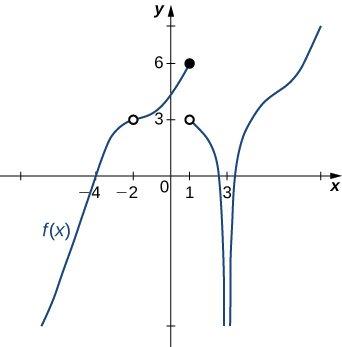
\includegraphics[width=0.5\textwidth]{../Figures/evaluateLimitGraphicallyCopyC.png}
\end{center}
\begin{enumerate}[label=\Alph*.]
\item \( -2 \)
\item \( -\infty \)
\item \( 1 \)
\item \( \text{Multiple } a \text{ make the statement true}. \)
\item \( \text{No } a \text{ make the statement true}. \)

\end{enumerate} }
\litem{
Based on the information below, which of the following statements is always true?
\begin{center}
    \textit{ $f(x)$ approaches $\infty$ as $x$ approaches $4$. }
\end{center}
\begin{enumerate}[label=\Alph*.]
\item \( f(x) \text{ is close to or exactly } 4 \text{ when } x \text{ is large enough}. \)
\item \( x \text{ is undefined when } f(x) \text{ is close to or exactly } \infty. \)
\item \( f(x) \text{ is undefined when } x \text{ is close to or exactly } 4. \)
\item \( f(x) \text{ is close to or exactly } \infty \text{ when } x \text{ is large enough}. \)
\item \( \text{None of the above are always true.} \)

\end{enumerate} }
\litem{
Evaluate the one-sided limit of the function $f(x)$ below, if possible.\[ \lim_{x \rightarrow -4^-} \frac{-9}{(x+4)^7}+6 \]\begin{enumerate}[label=\Alph*.]
\item \( -\infty \)
\item \( f(-4) \)
\item \( \infty \)
\item \( \text{The limit does not exist} \)
\item \( \text{None of the above} \)

\end{enumerate} }
\litem{
Evaluate the limit below, if possible.\[ \lim_{x \rightarrow 8} \frac{\sqrt{5x - 4} - 6}{3x - 24} \]\begin{enumerate}[label=\Alph*.]
\item \( \infty \)
\item \( 0.028 \)
\item \( 0.745 \)
\item \( 0.083 \)
\item \( \text{None of the above} \)

\end{enumerate} }
\litem{
Evaluate the limit below, if possible.\[ \lim_{x \rightarrow 7} \frac{\sqrt{5x - 10} - 5}{6x - 42} \]\begin{enumerate}[label=\Alph*.]
\item \( 0.017 \)
\item \( 0.100 \)
\item \( \infty \)
\item \( 0.373 \)
\item \( \text{None of the above} \)

\end{enumerate} }
\litem{
For the graph below, find the value(s) $a$ that makes the statement true: $ \displaystyle \lim_{x \rightarrow a} f(x) = -\infty$.
\begin{center}
    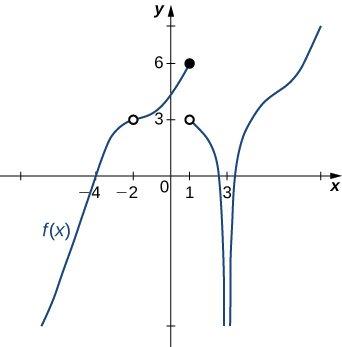
\includegraphics[width=0.5\textwidth]{../Figures/evaluateLimitGraphicallyC.png}
\end{center}
\begin{enumerate}[label=\Alph*.]
\item \( -\infty \)
\item \( 3 \)
\item \( -2 \)
\item \( \text{Multiple } a \text{ make the statement true}. \)
\item \( \text{No } a \text{ make the statement true}. \)

\end{enumerate} }
\end{enumerate}

\end{document}